\section{Наша Галактика: строение и основные параметры.}
\subsection{Основные сведения}
Галактика (Млечный Путь) -- спиральная галактика с перемычкой, в которой находится солнечная система. Млечный Путь вместе с галактикой Андромеды (М31), галактикой Треугольника (М33) и более чем 40 карликовыми галактиками-спутниками — своими и Андромеды — образуют Местную группу галактик которая входит в Местное сверхскопление (Сверхскопление Девы). 
\begin{figure}[H]
    \centering
    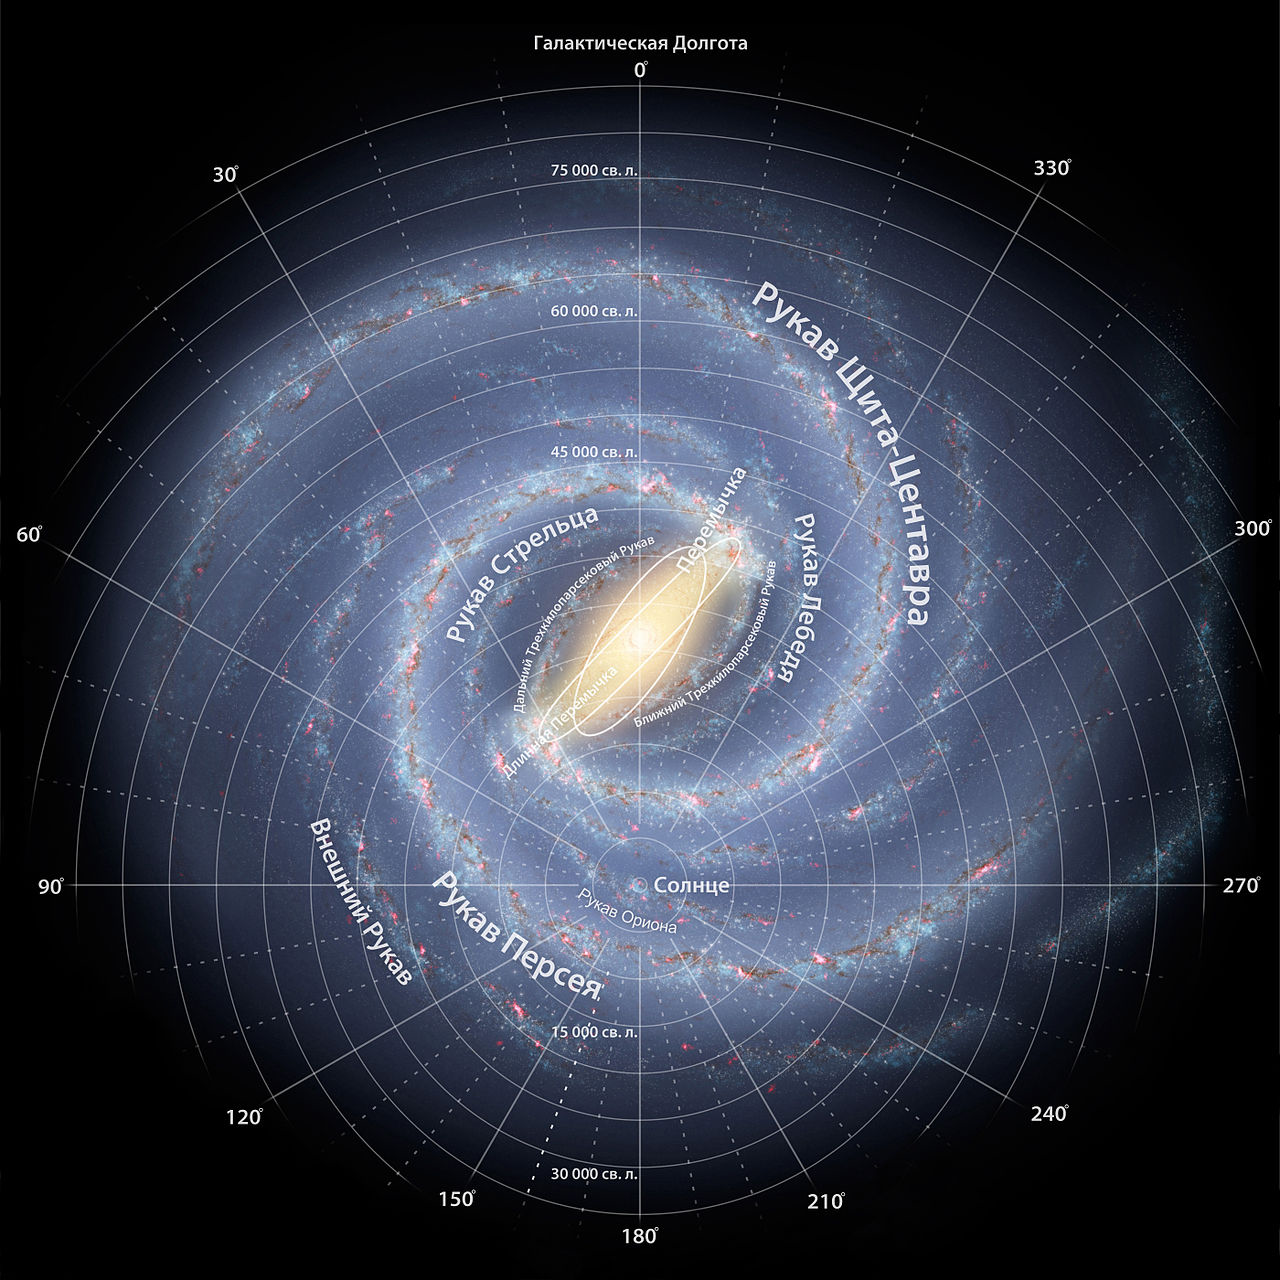
\includegraphics[scale=0.3]{15_galaxy.png}
    \caption{Рукава Млечного Пути.}
    \label{fig:galaxy_1}
\end{figure}
\subsection{Строение и параметры}
Млечный Путь — спиральная галактика с перемычкой («баром») из ярких звёзд, выходящей из центра и пересекающей галактику посередине. Спиральные ветви галактики начинаются на концах перемычки, тогда как в обычных спиральных галактиках они выходят непосредственно из ядра. Основные ветви (рукава) приведены на рисунке~\ref{fig:galaxy_1}.  
\begin{figure}[H]
    \centering
    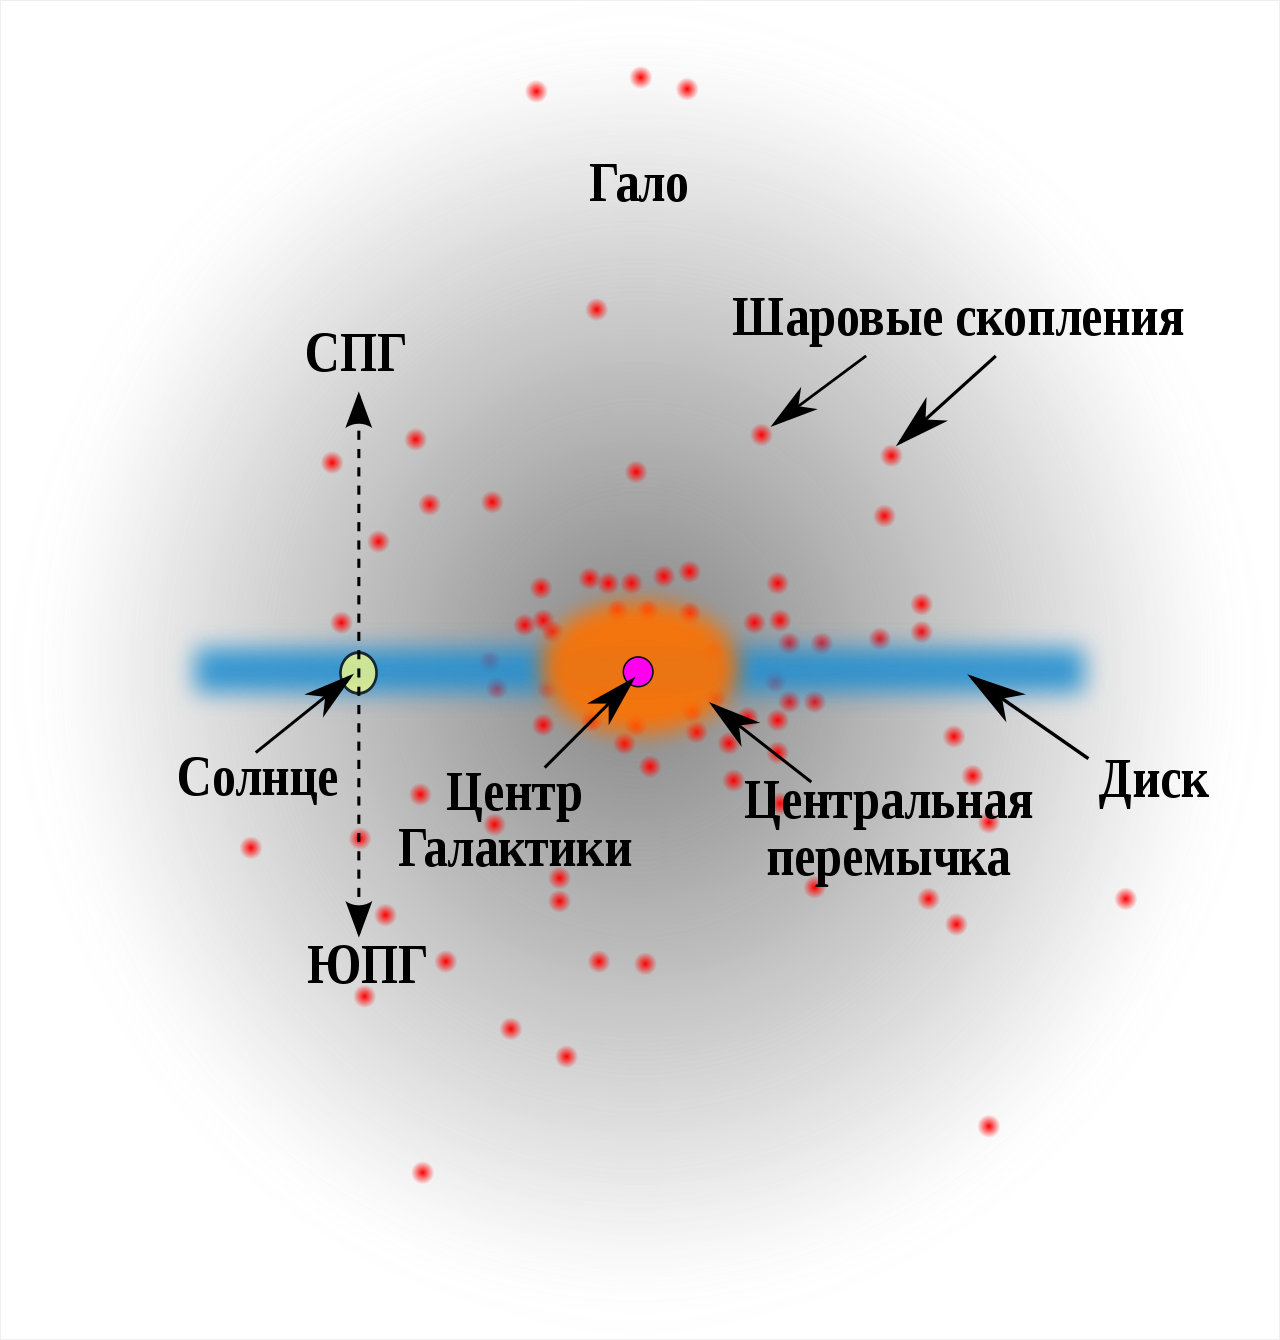
\includegraphics[scale=0.2]{15_galaxy_structure.png}
    \caption{Схематическое изображение структуры Галактики. ЮПГ и СПГ -- южный и северный полюса галактики.}
    \label{fig:galay_2}
\end{figure}
\subsubsection{Размеры}
Диаметр Галактики составляет около 30 тыс. парсек (порядка 100 000 световых лет, 1 квинтиллион километров), при оценочной средней толщине порядка 1000 световых лет.
\subsubsection{Количество звёзд}
Галактика содержит, по современной оценке, от 200 до 400 миллиардов звёзд. Их основная масса расположена в форме плоского диска.
\subsubsection{Масса}
Б\'{о}льшая часть массы Галактики содержится не в звёздах и межзвёздном газе, а в несветящемся гало из тёмной материи, поэтому точное определение массы Млечного Пути весьма затруднено.

В 2019 году, объединив новые данные миссий «Gaia» и «Hubble», астрономы определили, что масса Млечного Пути, в радиусе 129 000 световых лет от центра Галактики, составляет около $1.5\cdot10^{12}$ масс Солнца.
\subsubsection{Диск}
По оценкам учёных, галактический диск, выдающийся в разные стороны в районе галактического центра, имеет диаметр около 100 000 световых лет. По сравнению с гало, диск вращается заметно быстрее. Скорость его вращения неодинакова на различных расстояниях от центра. Она стремительно возрастает от нуля в центре до 200—240 км/с на расстоянии 2 тыс. световых лет от него, затем несколько уменьшается, снова возрастает примерно до того же значения и далее остаётся почти постоянной. Изучение особенностей вращения диска позволило оценить его массу, оказалось, что она в 150 млрд раз больше массы Солнца.

Вблизи плоскости диска концентрируются молодые звёзды и звёздные скопления, возраст которых не превышает нескольких миллиардов лет. Они образуют так называемую плоскую составляющую. Среди них очень много ярких и горячих звёзд. Газ в диске Галактики также сосредоточен в основном вблизи его плоскости. Он распределён неравномерно, образуя многочисленные газовые облака — от гигантских неоднородных по структуре облаков, протяжённостью свыше нескольких тысяч световых лет, к небольшим облакам размерами не более парсека.
\subsubsection{Центр Галактики}
В средней части Галактики находится утолщение, которое называется балджем, составляющее около 8300 парсек (27 000 световых лет) в поперечнике. Центр ядра Галактики находится в направлении Созвездия Стрельца ($\alpha = 265^{\circ}$, $\delta = - 29^{\circ}$). Расстояние от Солнца до центра Галактики 8500 парсек ($2.62\cdot10^{17}$ км, или 27 700 световых лет). В центре Галактики, по всей видимости, располагается сверхмассивная чёрная дыра (Стрелец $A^{*}$) (около 4,3 миллиона масс Солнца) вокруг которой, предположительно, вращается чёрная дыра средней массы от $1000M_{\Sun}$ до $10 000M_{\Sun}$ и периодом обращения около 100 лет и несколько тысяч сравнительно небольших. Их совместное гравитационное действие на соседние звёзды заставляет последние двигаться по необычным траекториям.

Для центральных участков Галактики характерна сильная концентрация звёзд: в каждом кубическом парсеке вблизи центра их содержатся многие тысячи. Расстояния между звёздами в десятки и сотни раз меньше, чем в окрестностях Солнца. Как и в большинстве других галактик, распределение массы в Млечном Пути такое, что орбитальная скорость большинства звёзд Галактики не зависит в значительной степени от их расстояния до центра. Далее от центральной перемычки к внешнему кругу обычная скорость обращения звёзд составляет 210—240 км/с. Такое распределение скорости, не наблюдаемое в Солнечной системе, где различные орбиты имеют существенно различные скорости обращения, является одним из указаний на существование тёмной материи.

Считается, что длина галактической перемычки составляет около 27 000 световых лет. Эта перемычка проходит через центр галактики под углом $44 \pm 10$ градусов к линии между нашим Солнцем и центром галактики. Она состоит преимущественно из красных звёзд, которые считаются очень старыми. Перемычка окружена кольцом, называемым «Кольцом в пять килопарсек». Это кольцо содержит большую часть молекулярного водорода Галактики и является активным регионом звездообразования в нашей Галактике. Если вести наблюдение из галактики Андромеды, то галактическая перемычка Млечного Пути была бы яркой его частью.
\subsubsection{}
Галактическое гало имеет сферическую форму, выходящую за пределы галактики на 5—10 тысяч световых лет, и температуру около $5\cdot105$ K. Галактический диск окружён сфероидным гало, состоящим из старых звёзд и шаровых скоплений, 90 \% которых находится на расстоянии менее 100 000 световых лет от центра галактики. Однако в последнее время было найдено несколько шаровых скоплений, таких как Pal 4 и AM 1, находящихся на расстоянии более чем 200 000 световых лет от центра галактики. Центр симметрии гало Млечного Пути совпадает с центром галактического диска. Состоит гало в основном из очень старых, неярких маломассивных звёзд. Они встречаются как поодиночке, так и в виде шаровых скоплений, которые могут содержать до миллиона звёзд. Возраст населения сферической составляющей Галактики превышает 12 млрд лет, его обычно считают возрастом самой Галактики.

В то время как галактический диск содержит газ и пыль, что затрудняет прохождение видимого света, сфероидная компонента таких составляющих не содержит. Активное звездообразование происходит в диске (особенно в спиральных рукавах, являющихся зонами повышенной плотности). В гало звездообразование завершилось. Рассеянные скопления также встречаются преимущественно в диске. Считается, что основную массу нашей галактики составляет тёмная материя, которая формирует гало тёмной материи массой примерно 600—3000 миллиардов масс Солнца. Гало тёмной материи сконцентрировано в направлении центра галактики.

Звёзды и звёздные скопления гало движутся вокруг центра Галактики по очень вытянутым орбитам. Так как вращение отдельных звёзд происходит несколько беспорядочно (то есть скорости соседних звёзд могут иметь любые направления), гало в целом вращается очень медленно.
\subsection{Положение Солнца в Галактике}
Согласно последним научным оценкам, расстояние от Солнца до галактического центра составляет $27 000 \pm 1 400$ световых лет, в то время как, согласно предварительным оценкам, наша звезда должна находиться на расстоянии около 35 000 световых лет от перемычки. Это означает, что Солнце расположено ближе к краю диска, чем к его центру. Вместе с другими звёздами Солнце вращается вокруг центра Галактики со скоростью 220—240 км/с, делая один оборот примерно за 200 млн лет. Таким образом, за всё время существования Земля облетела вокруг центра Галактики не более 30 раз.
